\section{Transpose}
\label{sec:transposel}

We present three algorithms for optimizing the transpose matrix operation.

The serial code for a transpose operation is presented in \cref{lst:transpose seq}.
The code loops through each index of the input, \ttt{h\_in[i, j]}, and copies the value to the transposed index in the output, \ttt{h\_out[j, i]}.
Given $n=width,\ m=height$This algorithm will take.
\begin{equation*}
workload: O(nm)
Steps: O(nm)
\end{equation*}

\begin{lstlisting}[caption={Serial transpose}, label={lst:transpose seq}]
void map(int *h_in, int *h_out, const int ROWS, const int COLUMNS) {
for(int row=0; row < ROWS; row++)
  for(int column=0; column < COLUMNS; column++)
    out[column + row*COLUMNS] = in[row + column*ROWS];
}
\end{lstlisting}

As we can analyse the problem as a mapping operation, as introduced in \cref{sec:challenges with parallel programs}, we know that every mapping operation is independant from one another why the amount of steps can be reduced to $O(1)$ and the problem thus becomes 100\% parallizible.

In \cref(lst:transpose elem) we present a trivial parallel implementation of the transpose algorithm.

\begin{lstlisting}[caption={Parallel transpose}, label={lst:transpose elem}]
__global__
void transpose_kernel(int * d_out, int * d_in,
                      const int ROWS, const int COLUMNS){
  int row = threadIdx.x + blockIdx.x * blockDim.x;
  int column = threadIdx.y + blockIdx.y * blockDim.y;
  if((row >= ROWS) || (column >= COLUMNS)) return;
  d_out[column + row*COLUMNS] = d_in[row + column*ROWS];
}
\end{lstlisting}

The dilemma with the trivial element-wise transpose presented in \cref(lst:transpose elem) is that the kernel will read row-wise but write column-wise.
The row-wise read will utilize coalesced reading whereas the writes will not be coalesced resulting in only one write per bus, wasting 48-4 bytes.
To utilize coalesced writes we present the tiled transpose in \cref(lst:transpose tiled).
The tiled transpose uses shared memory to make coalesced writes to global memory, such as introduced in \cref{sec:shared memory}.

\begin{lstlisting}[caption={Tiled transpose}, label={lst:transpose tiled}]
__global__
void transpose_kernel_tiled(int * d_out, int * d_in,
                            const int ROWS, const int COLUMNS){
  __shared__ int tile[DIM][DIM]; 
  int x = threadIdx.x + blockIdx.x * blockDim.x,
      y = threadIdx.y + blockIdx.y * blockDim.y;
  if((x >= COLUMNS) || (y >= ROWS)) return;
  tile[threadIdx.y][threadIdx.x] = d_in[x + y*COLUMNS];
  __syncthreads();
  x = threadIdx.x + blockIdx.y * blockDim.y;
  y = threadIdx.y + blockIdx.x * blockDim.x;
  d_out[x + y*ROWS] = tile[threadIdx.x][threadIdx.y];
}
\end{lstlisting}

The tiled solution, however, has memory bank conflicts such as described in \cref{sec:bank conflicts}.

\begin{figure}[htb]
  \centering
  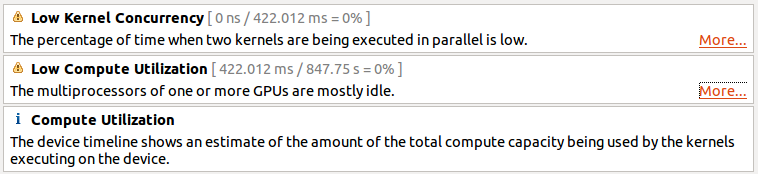
\includegraphics[width=.7\textwidth]{images/low-kernel-concurrency.png}
  \caption{nvidia Visual Profiler analysis indicates low kernel concurrency}
  \label{fig:first impl}
\end{figure}
